\documentclass[UTF8]{ctexart}
\usepackage{amsmath}
\usepackage{geometry}
\usepackage{float}
\geometry{left=3.0cm,right=3.0cm,top=3.0cm,bottom=3.0cm}

\begin{document}
%%%%%%%%%%%%%%%%%%%%%
\section{近似分布学习:算法与数值实验}
\subsection{近似分布学习}
\subsection{算法实现细节}
本次作业中,我们实现了经验重放的近似分布学习 Double DQN 算法,
在 OpenAI gym 环境下对 Atari 游戏 Alien 进行学习,
并与 OpenAI Baselines:DQN 算法在相同机器上进行了效果比较。
\par
我们实现的算法有如下值得提及的细节:
\begin{itemize}
\item 智能体在其生命周期内,分为三个行为阶段:观察阶段、探索阶段和学习阶段
            \footnote{该想法参考了 https://github.com/flyyufelix/C51-DDQN-Keras}。
    \begin{enumerate}
        \item 智能体的前 $N_{\text o}$ 个时间步为观察阶段。
                在这一阶段,智能体完全随机选择每一步的行动$a_t$,并将观测到的转换组
                $(\phi_t,a_t,r_t,\phi_{t+1})$ 存入重放缓存中。
                此时的智能体不进行网络的训练;
        \item 智能体在观察阶段后的 $N_{\text e}$ 个时间步内为探索阶段。
                在探索阶段,智能体仍然完全随机选择每一步的行动,并存储相应的转换组
                作为经验。但此时的智能体开始初步学习,训练网络;
        \item 智能体在探索阶段后进入训练阶段。
                此时的智能体按照 $\epsilon$-贪心方法选择动作$a_t$,仍然存储经验并训练网络。
                值得注意的是,在前两个阶段,随机选择行动 $a_t$ 相当于参数 $\epsilon=1$ 的
                $\epsilon$-贪心方法。在训练阶段,我们并不给定一个固定的 $\epsilon$ 值,而是以
                \[
                    \epsilon \leftarrow \epsilon_0 - \min {\left(1, \frac{ t-(N_{\text{o}}+N_{\text{e}})}
                       {f_{\text{e}}M}\right) \cdot (\epsilon_0 - \epsilon_{\min})}
                \]
                来确定 $\epsilon$。其中 $\epsilon_0=1$,$\epsilon_{\min}$ 为 $\epsilon$ 最小值,
                $N_{\text{o}}$ 和 $N_{\text{e}}$ 分别是观察和探索步数,
                $M$ 为最大行动步数,$f_{\text{e}}$ 为衰减系数。可见,$\epsilon$ 以线性方式由
                1 衰减至最小值 $\epsilon_{\min}$,而后保持不变。 
    \end{enumerate}
\item 值分布的支集 $\{z_i = V_{\min}+i\Delta z:0\leq i< N_{\text{atom}}\}$ 上的概率 $\{p_i(x,a)\}$ 由神经网络参数化,
        具体的网络结构如下:
        \begin{enumerate}
            \item 输入层:从环境 gym 中得到的游戏画面数据,图片像素的行数、列数和信道数随游戏而改变,
                样本数为 batch size 和记忆大小两者的较小值;
            \item 第一隐藏层:2维卷积层,filters=32,kernel\_size=(8,8),strides=(4,4),activation='relu';
            \item 第二隐藏层:2维卷积层,filters=64,kernel\_size=(4,4),strides=(2,2),activation='relu';
            \item 第三隐藏层:2维卷积层,filters=64,kernel\_size=(3,3),strides=(1,1),activation='relu';
            \item 第四隐藏层:Flatten层;
            \item 第五隐藏层:全连接层,units=256;
            \item 输出层:$N_a$ 个共享隐藏层的全连接层,每个全连接层的神经元数目 units=$N_{\text{atom}}$,激活函数
                    actication='softmax'。其中 $N_a$ 为从 gym 环境得到的当前游戏中全部可能行动的数目。
            \item [~]网络损失函数的形式为 categorical\_crossentropy。
        \end{enumerate}
\item 参数设置:
%\begin{table}[h]
%\centering
%\begin{tabular}{|c|c|c|}
%\hline
%		  		& Atlantis-v0 	& Alien-v0\\  \hline
%$V_{\min}$ 		& -400		& 0		\\ \hline
%$V_{\max}$	 	& 400		& 1000 	\\ \hline
%$N_{\text{atom}}$ 	& 51 			& 51		 \\ \hline
%$N_{\text o}$ 		& 1000 		& 10000	\\ \hline
%$N_{\text e}$ 		& 1000 		& 40000	 \\ \hline
%$M$				& 100000		& 500000	   \\ \hline
%$f_{\text e}$		& 0.1			& 0.2		   \\ \hline
%$\epsilon_0$		& 1			& 1		   \\ \hline
%$\epsilon_{\min}$	& 0.01		& 0.01	   \\ \hline
%$\gamma$		& 0.99		& 0.99	   \\ \hline
%\end{tabular}
%\end{table}
\begin{table}[h]
\centering
\begin{tabular}{|c|c|c|c|c|c|c|c|c|c|}
\hline

$V_{\min}$ &$V_{\max}$	&$N_{\text{atom}}$ &$N_{\text o}$ &$N_{\text e}$	&$M$&$f_{\text e}$	&$\epsilon_0$
&$\epsilon_{\min}$&$\gamma$\\ \hline
0& 1000 & 51& 10000& 40000	& 500000& 0.2& 1& 0.01& 0.99	 \\ \hline
\end{tabular}
\end{table}
\end{itemize}
\subsection{数值实验}
我们用来学习的硬件信息为:
\begin{itemize}
\item Intel(R) Core(TM) i7-4790 CPU@3.60GHz, 1物理处理器,4核心,8线程;
\item RAM:16GB
\item 无独立显卡
\end{itemize}
经过 578 个 episodes 的学习,近似分布学习方法的训练得分如下:
\begin{figure}[H]
\centering
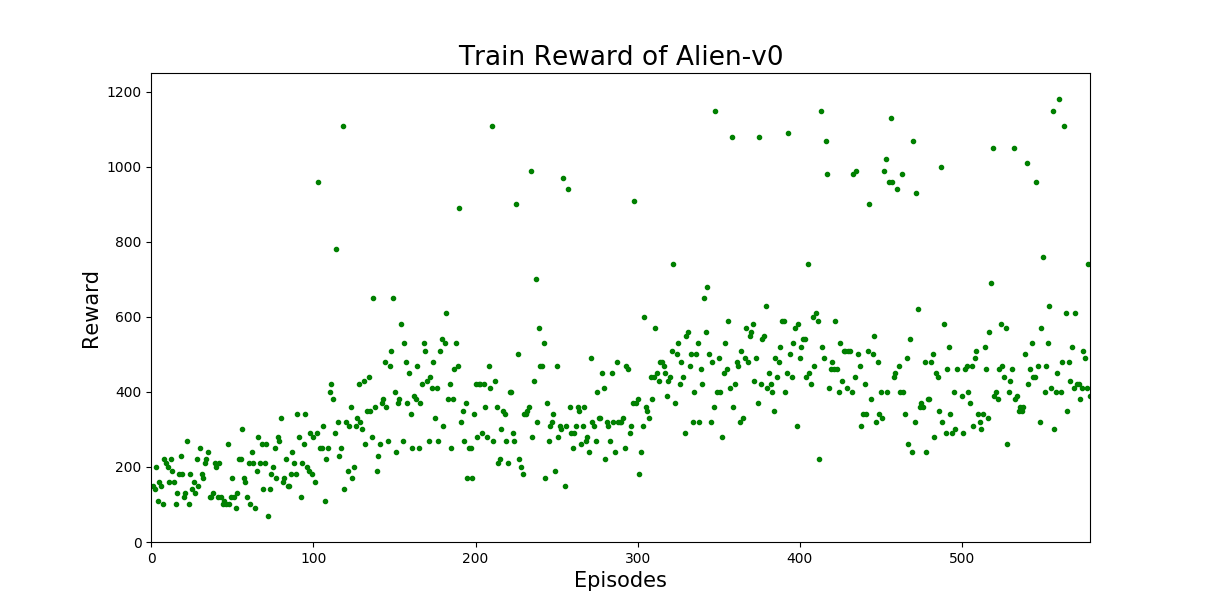
\includegraphics[scale=.55]{alien_train.png}
\end{figure}
智能体在 100 次测试中得分表现为:
\begin{figure}[H]
\centering
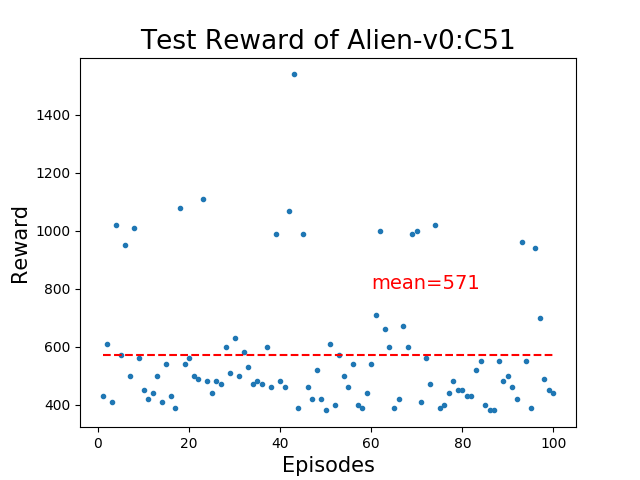
\includegraphics[scale=.8]{alien_c51.png}
\end{figure}
与随机行动时的得分相比,可见智能体的表现有着显著的提高:
\begin{figure}[H]
\centering
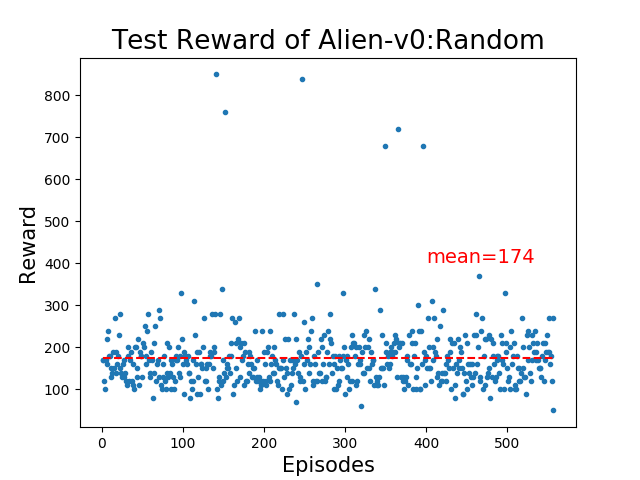
\includegraphics[scale=.8]{alien_random.png}
\end{figure}
从测试表现中可以看出,训练后的智能体得分分别集中在 500 分附近和 1000 分附近。通过观察游戏画面,我们发现,两个得分范围的差别主要在于游戏主角是否杀死过敌人。如果有更好的硬件设备进行更长时间的训练,我们有信心将测试平均分提升到 1000 分左右。
%%%%%%%%%%%%%%%%%%%%%
\end{document}
